\chapter{Outcome and Result}

\section{Simulation Result}

Building on the comprehensive test plan established earlier, this section delves into the simulation outputs to verify the pulse channel module's performance. The simulations compare the actual hardware responses against the theoretical predictions, ensuring that the module meets our strict design criteria for accuracy, reliability, and error detection. To thoroughly assess the module's behavior across a variety of conditions, a regression test from previous section was developed and executed. circumstances.

The regression test ran for over 1,000 iterations, with each iteration using a unique randomization seed that increments by one, starting at seed 1. This systematic variation in input ensures that the module is subjected to a broad spectrum of scenarios, helping to uncover any potential anomalies while confirming consistent performance. \autoref{table:error_results} offers an illustrative snapshot of the first ten iterations of this regression test, outlining several key performance metrics. The column labeled "Seed" denotes the specific randomization seed used during each iteration, providing insight into the exact conditions under which the test was conducted. The "Time" metric indicates the elapsed duration from when a pulse is triggered to when the corresponding error is detected. Additionally, the "Error/Delta" value represents the ratio between the observed error and the reference delta, offering a quantitative measure of performance discrepancies. The reference delta calculated by

\begin{equation}
delta = |Output_{current} - Output_{previous}|
\end{equation}

Finally, the "Pulse Number" specifies the sequential order of the pulse that produced the largest error-to-delta ratio during that iteration. Together, these detailed metrics enable us to thoroughly assess how the module responds under a wide spectrum of conditions, ultimately affirming its reliability and adherence to our stringent performance criteria.

\begin{table}[h]
\centering
\caption{Simulation results for first 10 seeds}
\begin{tabular}{|c|c|c|c|}
\hline
Seed & Time (ns) & Error/Delta & Pulse Number \\
\hline
1 & 159490 & 0.0035 & 3 \\
2 & 175960 & 0.1932 & 4 \\
3 & 189310 & 0.0096 & 5 \\
4 & 156640 & 0.0149 & 2 \\
5 & 159900 & 0.0022 & 2 \\
6 & 159090 & 0.3055 & 3 \\
7 & 161220 & 0.2224 & 3 \\
8 & 163910 & 0.1640 & 3 \\
9 & 134220 & 0.0164 & 0 \\
10 & 134220 & 0.0302 & 0 \\
\hline
\end{tabular}
\label{table:error_results}
\end{table}


\section{Board Result}
% TODO: need to collect something from the scope from 137 (Geoff's not good)
The system is examined using both an external hardware setup and Xilinx's Integrated Logic Analyzer (ILA). The external setup validates the overall functionality through peripheral interactions, while the ILA monitors internal signals from multiple modules, including the single pulse channel module.  This dual-method evaluation is essential to identify potential issues that simulations alone might overlook and to confirm that the system meets the rigorous performance standards expected in FPGA and computer architecture designs.
\begin{figure}[h]
    \centering
    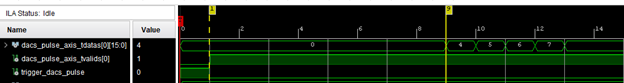
\includegraphics[width=1\linewidth]{figures/ila.png}
    \caption{ILA monitored the result (131,072 samples) from the top level.}
    \label{fig:ila}
\end{figure}
The ILA plays a crucial role in verifying the precise timing of waveform generation triggered externally. Traditional oscilloscopes often struggle to capture such high-resolution timing details, making the ILA essential for this role. For this experiment, a simple waveform—comprising the sequence 4, 5, 6, and 7 starting at the earliest possible time—is fed into the hardware. The result measures the delay between the external trigger and the first output by monitoring channel 0 at the top-level CC-P, specifically noting when the value 4 is emitted. As illustrated in \autoref{fig:ila}, the first output appears after 8 cycles, with each cycle lasting 10 nanoseconds. This timing results in an 80-nanosecond delay, confirming that the pulse generation operates well within the sub-microsecond range required for quantum control hardware. Furthermore, the ILA data shows that data updates occur every 10 nanoseconds, demonstrating the rapid switching performance essential for high-speed applications. Such precise control and measurement are critical for ensuring that the system meets the rigorous demands of modern FPGA-based designs and quantum control systems.

\section{Resource Utilization}

In FPGA design, efficient resource utilization is essential for ensuring a high-quality, reliable system. One of the most critical aspects of this evaluation is timing analysis. After implementation, the Xilinx Vivado tool generates an in-depth timing report that details the minimum and maximum delay paths within the design. As shown in \autoref{fig:sta}, the report confirms that the critical timing parameters—both setup and hold times—meet the specified constraints.
\begin{figure}[h]
    \centering
    
\includegraphics[width=1\linewidth]{figures/timimg_report.png}
    \caption{Partial timing report from Vivado on the worst slack (top) and hold (bottom).}
    \label{fig:sta}
\end{figure}
This timing verification is crucial because it ensures that all synchronous elements operate correctly within the designated clock cycle, preventing data corruption and operational failures. By analyzing these delay paths, designers can identify potential bottlenecks and optimize the design to maintain system stability. In essence, the successful meeting of timing requirements signifies that the design can perform reliably under its intended operating conditions, making it suitable for high-speed FPGA applications.

\autoref{table:util} presents the post-implementation power consumption and resource utilization data from Vivado. The report shows that only a small fraction of the FPGA resources is used. This low usage proves the design is highly efficient. It leaves plenty of headroom for future enhancements. Minimal resource usage reduces power consumption. It also helps the FPGA maintain optimal timing and routing. This efficiency is ideal for scalable systems that may need future modifications. It validates the careful design decisions made during synthesis and optimization.

\begin{table}
    \centering
    \begin{tabular}{|l|r|r|r|r|}
    \hline
    \textbf{On-Chip} & \textbf{Power (W)} & \textbf{Used} & \textbf{Available} & \textbf{Utilization (\%)} \\
    \hline
    Clocks & 0.017 & 3 & --- & --- \\
    CLB Logic & 0.004 & 10028 & --- & --- \\
    ~~LUT as Logic & 0.004 & 3718 & 274080 & 1.36 \\
    ~~Register & $<$0.001 & 5092 & 548160 & 0.93 \\
    ~~CARRY8 & $<$0.001 & 69 & 34260 & 0.20 \\
    ~~LUT as Shift Register & $<$0.001 & 4 & 144000 & $<$0.01 \\
    ~~Others & 0.000 & 297 & --- & --- \\
    Signals & 0.006 & 7974 & --- & --- \\
    Block RAM & 0.024 & 38 & 912 & 4.17 \\
    DSPs & $<$0.001 & 2 & 2520 & 0.08 \\
    I/O & 0.011 & 29 & 328 & 8.84 \\
    PS8 & 2.472 & 1 & --- & --- \\
    Static Power & 0.748 & & & \\
    ~~PS Static & 0.098 & & & \\
    ~~PL Static & 0.651 & & & \\
    Total & 3.283 & & & \\
    \hline
    \end{tabular}
    \caption{Resource Utilization Reported from Vivado}
    \label{table:util}
\end{table}